\documentclass[12pt, a4paper, oneside]{article}
\usepackage{amsmath, amsthm, amssymb, bm, graphicx, hyperref, mathrsfs}

\title{\textbf{Assignment\#2 CS305 Fall 2023}}
\author{Ben Chen(12212231)}
\date{\today}
\linespread{1.3}
\newcounter{problemname}
\newenvironment{problem}{\stepcounter{problemname}\par\noindent\textsc{Problem \arabic{problemname}. }}{\\\par}
\newenvironment{solution}{\par\noindent\textsc{Solution. }}{\\\par}
\newenvironment{note}{\par\noindent\textsc{Note of Problem \arabic{problemname}. }}{\\\par}

\begin{document}

\maketitle

\begin{problem}
    Answer the questions related to UDP checksum with the 32-bit word transmitted
    \begin{equation*}
        01100110011000000101010101010101
    \end{equation*}
\end{problem}

\begin{solution}
    \textbf{a)} Break the word into 16 bits
    \begin{align*}
        \textit{Word}_1 &= 0110011001100000 \\
        \textit{Word}_2 &= 0101010101010101
    \end{align*}
    And their 1's complements are
    \begin{align*}
        \textit{Word}_1^{\ \prime} &= 1001100110011111 \\
        \textit{Word}_2^{\ \prime} &= 1010101010101010 \\
        \textit{checksum} &= 0100010001001010
    \end{align*}
    \textbf{b)} The receiver verifies the message by checking the sum of segments of 16 bits
    \begin{align*}
        \textit{result} &= \textit{Word}_1 + \textit{Word}_2 + \textit{checksum} \\
                        &= 1111111111111111
    \end{align*}
    If the bits of result are 1, then no error detected. Otherwise there must be errors.
    \newline\textbf{c)} No, the message might have errors, for example considering the corrupted message
    \begin{align*}
        \textit{Word}_1 &= 0110011001100001 \\
        \textit{Word}_2 &= 0101010101010100
    \end{align*}
    say, if the least bits of Word1 and Word2 exchanged, the checksum cannot detect the error.
\end{solution}

\begin{problem}
    In a TCP connection, Fill in the blanks (B1) and (B2) in the below figure for go-back-N and selective repeat.
\end{problem}

\begin{solution}
    \textbf{a)} (B1) resend \textbf{ack0} (B2) 01\ \boxed{234}\ 56
    \newline\textbf{b)} (B1) send \textbf{ack2} (B2) 0123\ \boxed{456}
\end{solution}

\begin{problem}
    Suppose that instead of multiplicative decrease, TCP decreased the window size by a constant amount. Would the resulting AIAD algorithm converge to an equal share algorithm?
\end{problem}

\begin{solution}
    No, the AIAD algorithm will never converge to an equal share algorithm since the rates are limited to their initial rates $X$ and $Y$
    \begin{figure}[!htbp]
        \begin{center}
            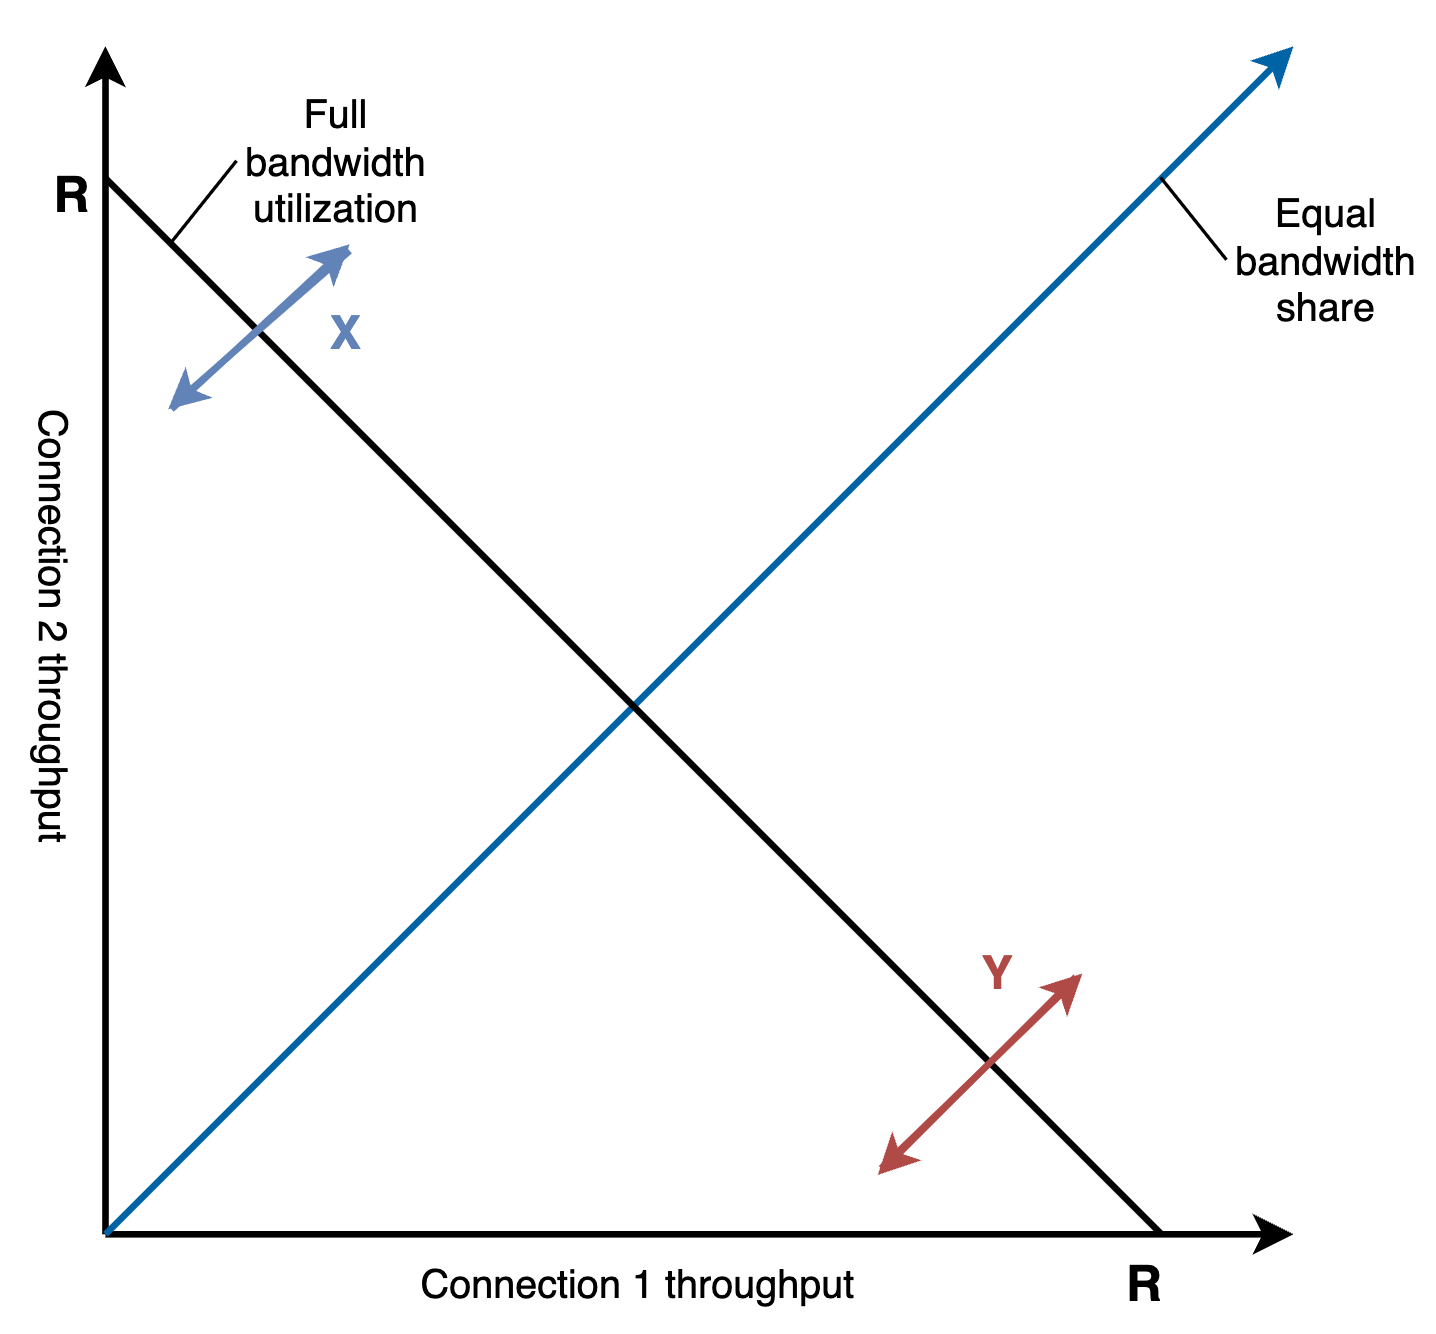
\includegraphics[width=0.5\textwidth]{cong.png}
        \end{center}
    \end{figure}
\end{solution}

\begin{problem}
    Draw the TCP connection-establishment procedure between a client host and a server host with the initial sequence number of the client host is $25$, and that of the server host is $89$.
\end{problem}

\begin{solution}
    The figure is shown below, only the third segment can carry payload while the first two segments cannot send data.
    \begin{figure}[!htbp]
        \begin{center}
            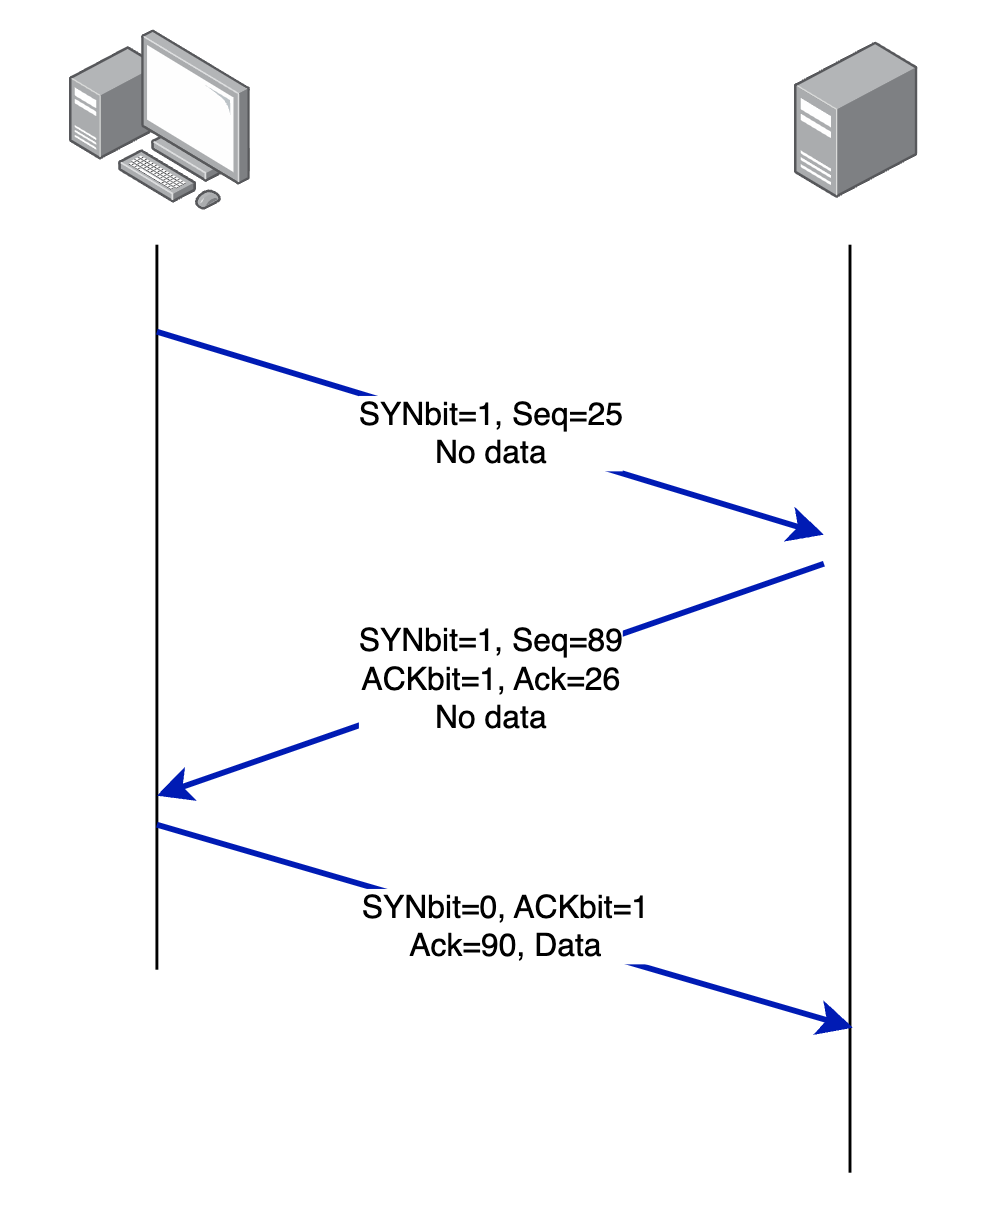
\includegraphics[width=0.75\textwidth]{tcp.png}
        \end{center}
    \end{figure}
\end{solution}

\begin{problem}
    Consider the TCP procedure for estimating RTT. Suppose that $\alpha = 0.1$, and \textit{EstimatedRTT} is initialized as $\textit{EstimatedRTT}_0$. Recall that\[\textit{EstimatedRTT} = (1 - \alpha)\textit{EstimatedRTT} + \alpha \textit{SampleRTT}\]
\end{problem}

\begin{solution}
    \textbf{a)} The \textit{EstimatedRTT} is
    \begin{align*}
        &= 0.9\cdot\textit{EstimatedRTT}_0 + 0.1\cdot\textit{SampleRTT}_1 \\
        &= 0.81\cdot\textit{EstimatedRTT}_0 + 0.09\cdot\textit{SampleRTT}_1 + 0.1\cdot\textit{SampleRTT}_2 \\
        &= 0.729\cdot\textit{EstimatedRTT}_0 + 0.081\cdot\textit{SampleRTT}_1 + 0.09\cdot\textit{SampleRTT}_2 + 0.1\cdot\textit{SampleRTT}_3 \\
        &= 0.6561\cdot\textit{EstimatedRTT}_0 + 0.0729\cdot\textit{SampleRTT}_1 + 0.081\cdot\textit{SampleRTT}_2 \\ &\quad + 0.09\cdot\textit{SampleRTT}_3  + 0.1\cdot\textit{SampleRTT}_4
    \end{align*}
    \textbf{b)} From the patterns above, it's obvious that for $n$ sample RTTs we have
    \begin{align*}
        \textit{EstimatedRTT} &= 0.9^n \textit{EstimatedRTT}_0 + 0.1\cdot\sum_{i=1}^n 0.9^{n-i}\textit{SampleRTT}_i
    \end{align*}
\end{solution}

\end{document}
